\documentclass[hidelinks, 12pt, oneside]{article}
\usepackage{bookmark}
\usepackage{graphicx}
\usepackage{hyperref}
\usepackage{titlesec}
\setcounter{secnumdepth}{4}
\usepackage[utf8]{inputenc}
\usepackage[english]{babel}


\begin{document}

	\begin{center}
    \centering
    
%University logo
    
\includegraphics[width=144px]{img/icon.png}
    \rule{0\linewidth}{0.15\linewidth}\par
    
    		\begin{center}
		{\uppercase{\Large User Manual\par}}
   		{\Large iCrawler \par}
   			\vspace{1cm} 
   		{\Large Emilio Mumba  \par} 
    		\vspace{1cm}
		   		
    		{\Large The 5 Concurrent Nodes \par} 
    		\vspace{1cm}
		
		{\normalsize Khathutshelo Shaun Matidza\par}
		{\normalsize Sylvester Sandile Mpangane\par}
		{\normalsize Thabang Michael Letageng\par}
		{\normalsize Matthew Nel\par}
		
		\end{center}

		\textbf{}		
		\centering
		\vspace{2cm}
		Department of Computer Science, University of Pretoria

		
	 	{\Large  September 2015}
\end{center}
\clearpage


	\tableofcontents
	\newpage
	\section{Vision and Scope}
	\subsection{Project Vision}
	\vspace{0.3 cm}
	  Digital forensics is defined as the use of scientifically derived and proven methods towards the preservation, collection, validation, identification, analysis, interpretation and presentation of digital evidence derived from digital sources for the sole purpose of facilitating or furthering the reconstruction of events found to be criminal or helping to anticipate the unauthorized actions shown to be disruptive to planned operations [3].
Readiness is considered as the process of being prepared for a digital investigation before an incident has occurred [2]. \newline\newline
The proposal of a mobile monitoring application will promote readiness in digital forensics and protect mobile users from malicious entities and activities. It aims to provide a proactive measure that is undertaking by the mobile device user or mobile device owner. Having this application installed on mobile devices will proactively ensure that relevant digital evidence is made ready and available before an incident occurs. The mobile monitoring application is expected to monitor user activities on a mobile device and report application data/logs to a dashboard on a desktop computer. It will generate reports giving the investigator quick and comprehensive data/logs that provide a starting point during a mobile device investigation. \newline\newline
The objective of the mobile monitoring application is to collect data/logs and assist in understanding the activities performed by a mobile user as well as shedding more light into the behaviour of the mobile user. Combining activities from the various applications promotes a proactive approach which in turn enforces proactive (readiness) measures. 
	\subsection{Project Scope}
		{\centering
		
		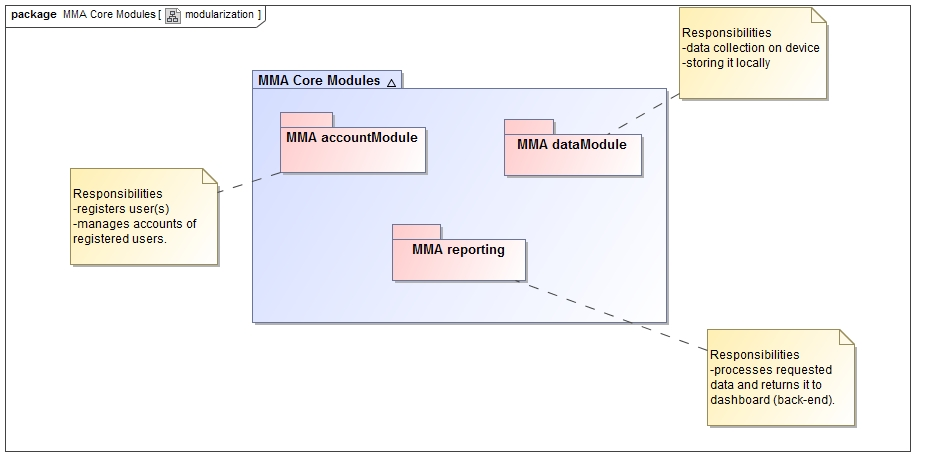
\includegraphics[width=400px,height=220px]{img/highLevelSystem.jpg}
		\newline
		Figure 1: High level system modules
		\newline\newline
		The high level modules of the Mobile Monitoring App is as indicated on figure 1 above. The responsibilities of each module are also noted.
		}
	
	\section{Application Requirements and Design}
	The following section will explain each module in the Mobile Monitoring App. It will discuss the use-case design and  functional requirements extracted from the use-case; along with the selected service contracts.\newline
	
	\subsection{Modular System}
	 The application is going to use a modular design. This will allow the following:
	 \begin{itemize}
	\item add new functionality in the future
 	\item decouple the system
	\end{itemize}


	
	\subsection{MobileMonitoringApp - Accounts module}
	%You will have to elaborate on what the module does (look at the high level module notes for help)
	\subsubsection{Scope}
	%The width and height of the image should not be changed. Just uncomment the line below and specify img source
	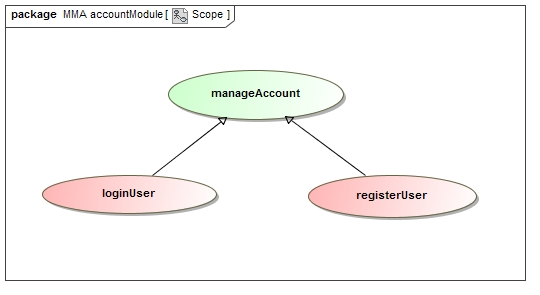
\includegraphics[width=400px,height=220px]{img/scopeAccounts.jpg}
		Figure : Scope of mmaAccounts module
	\subsubsection{Use-Cases}
		This section provides details on the use-case requirements for the use-cases offered by this module.
	\paragraph{registerUser - priority: important}
		This use-case registers a user on initial installation after user accepts terms and conditions of use.\newline
	\paragraph{loginUser - priority: important}
		This use-case logins a user on initial installation after user accepts terms and conditions of use.\newline	
	\subparagraph{Service Contract}
		The service contract for registerUser is shown in the figure below. The pre-conditions are enforced (raises an exception if not met) and on
		success the user is registered and the device and user data is persisted through the local database.\newline
	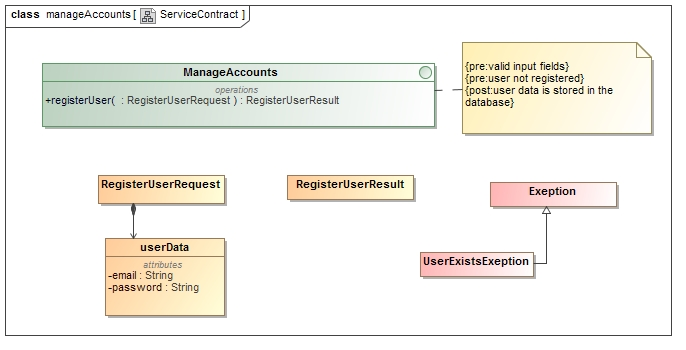
\includegraphics[width=400px,height=220px]{img/serviceContractRegisterUser.jpg}
		Figure : The service contract for registering a new user on the app\newline
	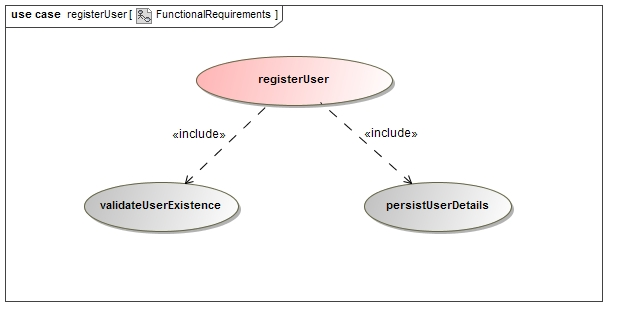
\includegraphics[width=400px,height=220px]{img/functionalRequirementsRegister.jpg}
		Figure : The functional requirements for registerUser\newline
	
	
	
	\subsection{MobileMonitoringApp - Data module}
	%You will have to elaborate on what the module does (look at the high level module notes for help)
	\subsubsection{Scope}
		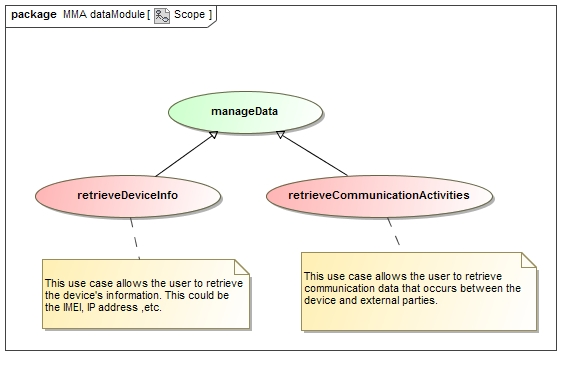
\includegraphics[width=400px,height=220px]{img/scopeData.jpg}
		Figure : Scope of MMA dataModule	
		
		
	
	\subsubsection{Use-Cases}
		This section provides details on the use-case requirements for the use-cases offered by this module.	
		
	\paragraph{retrieveDeviceInfo - priority: important}
		The retrieveDeviceInfo use case retrieves all the relevant device information from the device.\newline
	\paragraph{retrieveCommunicationActivities - priority: important}
		The retrieveCommunicationAcitivites use-case retrieves all the users communication activities from the various apps on the device.\newline
\subparagraph{Service Contract}
		The service contract for manageData is shown in the figure below. The retrieveCommunicationActivitiesRequest requests the data regardless of the data type and retrieveCommunicationActivitiesRequest retrieves the data where it packages the data and stores it on the database locally.\newline\newline	
	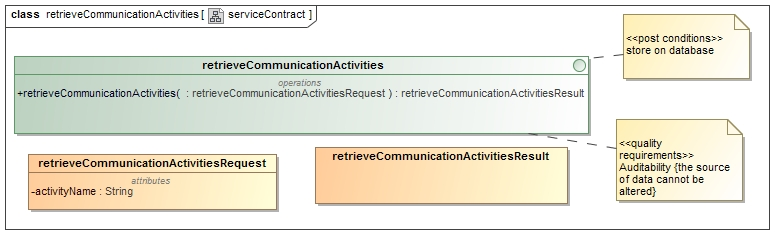
\includegraphics[width=400px,height=220px]{img/serviceContractRetrieveCommunicationActivities.jpg}
		Figure : The service contract for manage data on the device\newline
	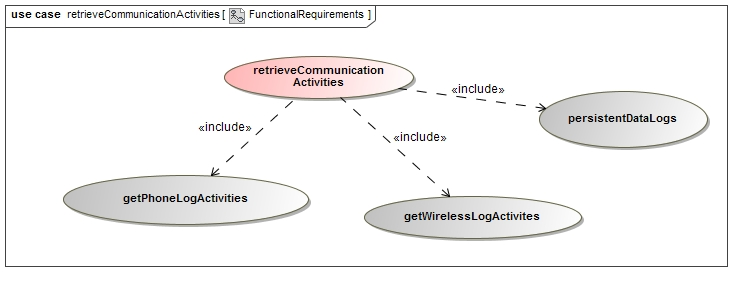
\includegraphics[width=400px,height=220px]{img/functionalRequirementsRetrieveCommunicationActivities.jpg}
		Figure : The functional requirements for retrieveCommunicationActivities\newline
	
	
	\subsection{MobileMonitoringApp - Reports module}
	%You will have to elaborate on what the module does (look at the high level module notes for help)
	\subsubsection{Scope}
	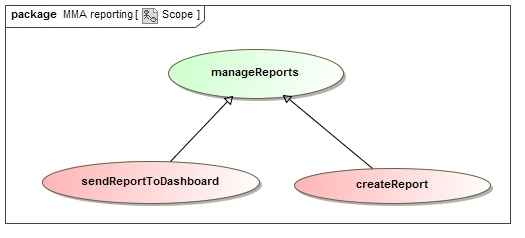
\includegraphics[width=400px,height=220px]{img/scopeReports.jpg}
			Figure : Scope of mmaReporting module
	\subsubsection{Use-Cases}
			This section provides details on the use-case requirements for the use-cases offered by this module.
		\paragraph{ createReport - priority: important}
		This use-case retrieves logs from the device.
		\paragraph{ sendReportToDashboard - priority: important}
		This module sends the report onto a server where they will be saved on a database to de displayed later on a dashboard .\newline
		\subparagraph{Service Contract}
			The service contract for sendReportToDashboard is shown in the figure below. The pre-condition is not enforced i.e. If the app fails to estabilish a connection with the server, the report will be saved temoparily on the device until a connection is estabilished.\newline
		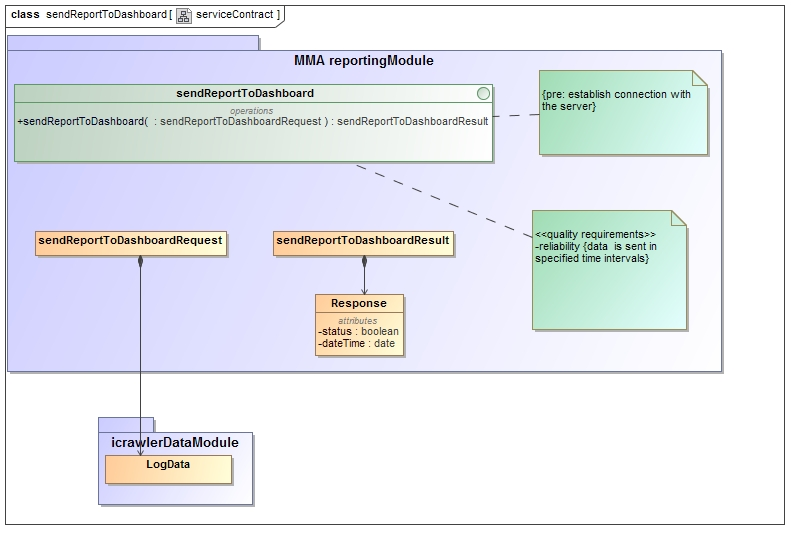
\includegraphics[width=400px,height=220px]{img/serviceContractSendReportToDashboard.jpg}
			Figure : The service contract for sendReportToDashboard\newline \newline \newline
		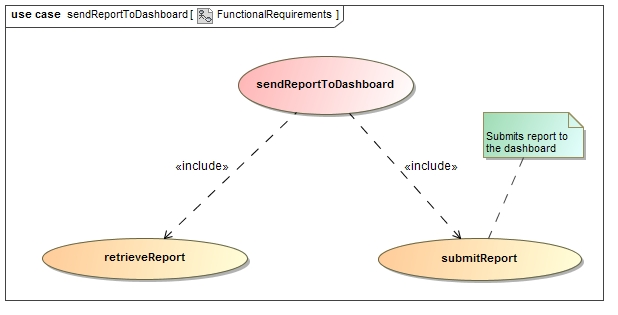
\includegraphics[width=400px,height=220px]{img/functionalRequirementsSendReportToDashboard.jpg}
			Figure : The functional requirements for sendReportToDashboard\newline	
\end{document}
